\documentclass{article}
\usepackage{amsmath}
\usepackage{amsthm}
\usepackage{amssymb}
\usepackage{amsfonts}
\usepackage{mathtools}
\usepackage{listings}
\title{MATH 620: Homework 5}
\author{Fernando}
\date{\today}
\begin{document}
\maketitle
\section*{Problem 1}
\subsection*{Part 1}
According to the definition we need that
\[
	\int u \phi' = -\int g \phi
\]
for every bump function $\phi$.

First we can see that $g\equiv 0$ on $(-\infty,0)$ because $u$ is constant
there. Same argument shows that $g\equiv 0$ on $(0,\infty)$, then
$g\equiv 0$, which means that $\int u \phi' = 0$ for all bump
functions $\phi$. But this is clearly not true because the fundamental theorem
of variations would imply that $u=0$. Another way to see that this is false is
taking a specific bump function, for example $e^{-1/(1-x^2)}$. According to
Wolfram Alpha its derivative looks like this:

\begin{center}
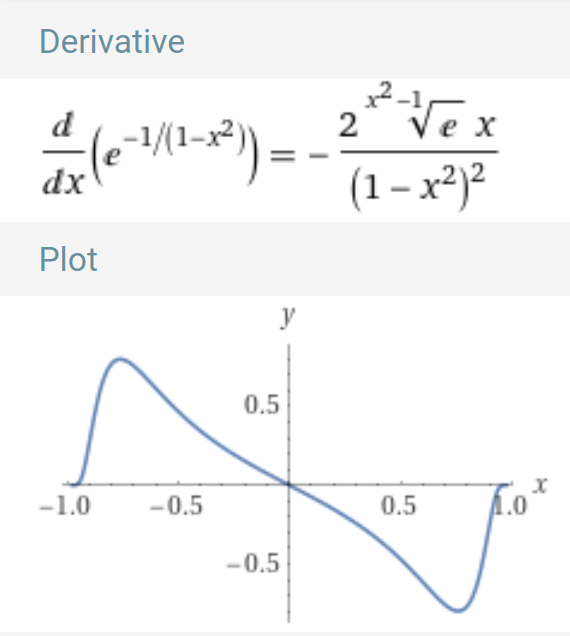
\includegraphics[width=0.5\textwidth]{bumpPrime.png}
\end{center}

Then multiplying by $u$ kills everything after 0 and multiplies by -1 the part
before 0. If we integrate that, the result is clearly not 0.
\subsection*{Part 2}
We want to find $g$ such that
\[
	\int u |\nabla \phi| = -\int g \phi
\]
for all bump functions $\phi$.

Following the suggestion we change to polar coordinates.
Then $u$ becomes:
\[
u(\theta)=\sin(\arctan(\tan(\theta)))=\begin{cases}
	\sin(\theta) \quad \text{for } -\frac{\pi}{2} < \theta < \frac{\pi}{2}\\
	-\sin(\theta) \quad \text{for } \frac{\pi}{2} < \theta < \frac{3\pi}{2}
\end{cases}
\]
and we want to find $g$ such that
\[
	\int_{B_1(0)}ru\phi'=\int_{B_1(0)}rg\phi
\]
for all bump functions $\phi$.
Intuitively the weak derivative should be
\[
g(\theta)=\begin{cases}
	\cos(\theta) \quad \text{for } -\frac{\pi}{2} < \theta < \frac{\pi}{2}\\
	-\cos(\theta) \quad \text{for } \frac{\pi}{2} < \theta < \frac{3\pi}{2}
\end{cases}.
\]
Now let's prove it
\begin{align*}
	\int_{B_1(0)}ru\phi' &=\int_{-\frac{\pi}{2}}^{\frac{\pi}{2}} \int_0^1 r\sin(\theta)\phi'drd\theta\\
		      &+\int_{\frac{\pi}{2}}^{\frac{3\pi}{2}} \int_0^1 r\sin(\theta)\phi'drd\theta\\
		      &= \int_{-\frac{\pi}{2}}^{\frac{\pi}{2}}\sin(\theta) \int_0^1 r\phi'drd\theta\\
	  	      &+ \int_{\frac{\pi}{2}}^{\frac{3\pi}{2}}\sin(\theta) \int_0^1 r\phi'drd\theta
\end{align*}
\section*{Problem 2}
Let $\varphi$ be a linear functional. We have to prove that $\varphi$ is continuous
iff $\varphi$ is bounded.
\subsection*{continuous $\implies$ bounded}
First notice that if $||x||_X=0$ then $x=0$ by properties of the norm and since
$\varphi$ is linear $\varphi(x)=\varphi(0)=0$ and the inequality is trivially true. Now
we can consider $x\neq0$. Then the inequality is equivalent to:
\[
	\bigg|\varphi\left(\frac{x}{||x||_X}\right)\bigg| \leq c
\]
where we used the fact that $\varphi$ is linear. Now because $\varphi$ is
continuous by hypothesis and so is the absolute value their composition is
continuous.
\subsection*{bounded $\implies$ continuous}
Let $x_k \to x$ i.e. $||x_k-x||_X \to 0$ as $k \to \infty$. By hipothesis
\[
	|\varphi(x_k-x)|\leq c ||x_k-x||_X
\]
so $\varphi(x_k-x) \to 0$ as $k \to \infty$.

\section*{Problem 3}
\section*{Problem 4}
\section*{Problem 5}
\end{document}
